\documentclass{article}

\usepackage{graphicx} %package to manage images
\graphicspath{ {./images/} }

\usepackage[rightcaption]{sidecap}

\usepackage{wrapfig}

\begin{document}


\title{Explicación Modificacion del algoritmo Sample Mean Reversion de Quantopian}
\author{Alex Jose Alberto Barreto Cajica\\ 
Algoritmos 2019 - 2}
\maketitle
En este algoritmo se plantea trabajar vendiendo el 10\% de las compañías con mejores retornos y comprar las 10 con peores.\\ El proceso que seguí para realizar las modificaciones para encontrar la mejor rentabilidad fueron cambiar valores de la ventana de tiempo en que se analiza, también con qué frecuencia se realiza la operación, en este caso lo definí como mensual y elegí un día especifico para realizar la transacción y también cambie la concentración que se tenía sobre cada Stock que según mi análisis es una de las variables más sensibles que presenta el código y así mismo puede ver que una de las cosas que es menos sensible se puede decir que insensible para este código es el porcentaje de empresas que se compran que las que se vende teniendo siempre el equilibrio entre estas.\\ 
Finalmente encontré una buena configuración que me permite tener un retorno total en los dos años de 16.6\%\\



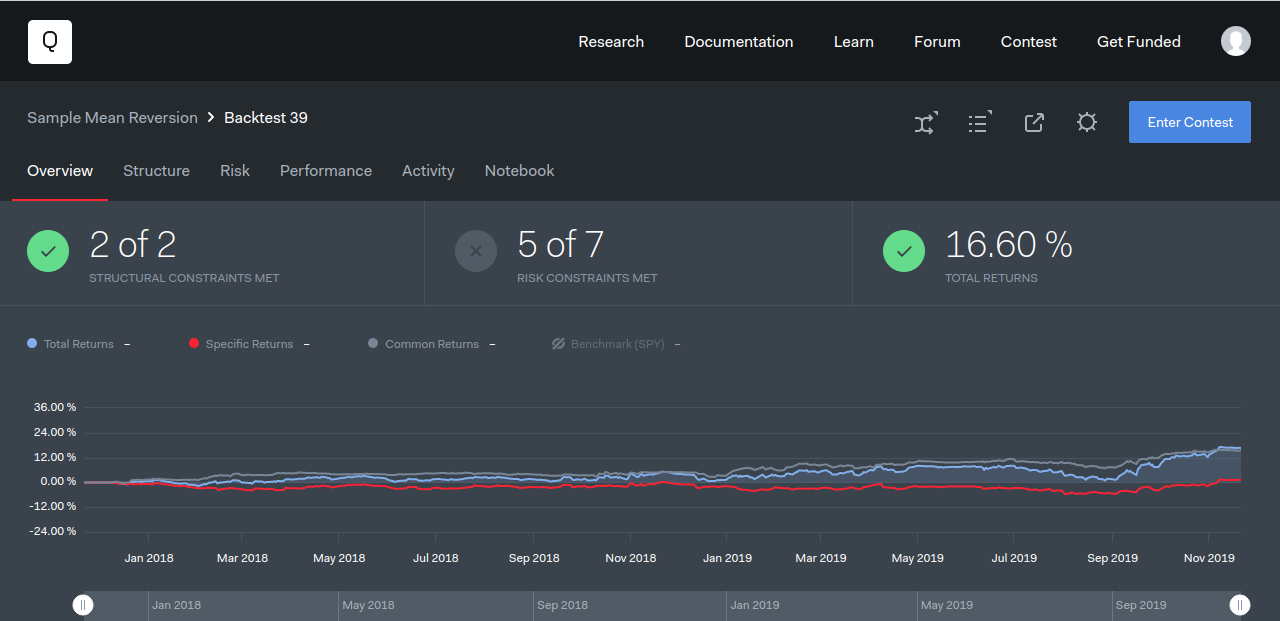
\includegraphics[width=\textwidth]{QT.png}
\href{https://www.quantopian.com/posts/sample-mean-reversion-2}



\end{document}


